The shuffled complex evolution is a population
based evolutionary optimization algorithm that regards a natural 
evolution happening simultaneously in independent communities.
The algorithm works with a population partitioned in $N$ complexes, each one
having $M$ individuals.
In the next Subsection the SCE is explained in more details.
In the later Subsection the application of SCE to the multidimensional knapsack
problem is considered.
% In the SCE the population is partitioned into communities (complexes), each of which
% will evolve independently through a number of evolving steps.
% In each evolving step a subset of the complex (subcomplex) is selected as potencial group of
% parents.

%To avoid been trapped in local optimum a new offspring can be occasionally taken
%from a random location of the feasible space and introduced to the complex.

\subsection{The shuffled complex evolution}
In the SCE a population of $N*M$ individuals is randomly taken from the
feasible solution space.
After this initialization the population is sorted by descending order according
to their fitness and the best global solution is identified.
The entire population is then partitioned (shuffled) into $N$ complexes,
each containing $M$ individuals.
In this shuffling process the first individual goes to the first complex, the second
individual goes to the second complex, individual $N$ goes to $N$-th complex,
individual $M+1$ goes back to the first complex, etc.

The next step after shuffling the complexes is to evolve each complex through
a given fixed amount of $K'$ steps.
The individuals in each complex is sorted by descending order of fitness quality.
In each step a subcomplex of $P$ individuals is selected from the
complex using a triangular probability distribution, where the $i$-th individual
has a probability $p_i = \frac{2(n+1-i)}{n(n+1)}$ of being selected.
The use of triangular distribution is intended to prioritize individuals with
better fitness, supporting the algorithm convergence rate.

After the selection of the subcomplex, its worst individual is identified to
be replaced by a new generated solution.
This new solution is generated by the crossing of the worst individual and an
other individual with better fitness.
At first the best individual of the subcomplex is considered for the crossing.
If the new solution is not better than the worst one, the best individual
of the complex is considered for a crossing.
If the latter crossing did not result in any improvement, the best individual
of whole population is considered.
Finally, if all the crossing steps couldn't generate a better individual,
the worst individual of the subcomplex is replaced by a new random solution taken
from the feasible solution space.
This last step is important to prevent the algorithm becoming trapped in local minima.
Fig.~\ref{fig:flow2} presents the evolving procedure described above in a flowchart diagram.

After evolving all the $N$ complexes the whole population is again
sorted by descending order of fitness quality and the process continues until
a stop condition is satisfied.
Fig.~\ref{fig:flow1} shows the SCE algorithm in a flowchart diagram.

\begin{figure}[t]
  \subfigure[The SCE algorithm overview.]{
    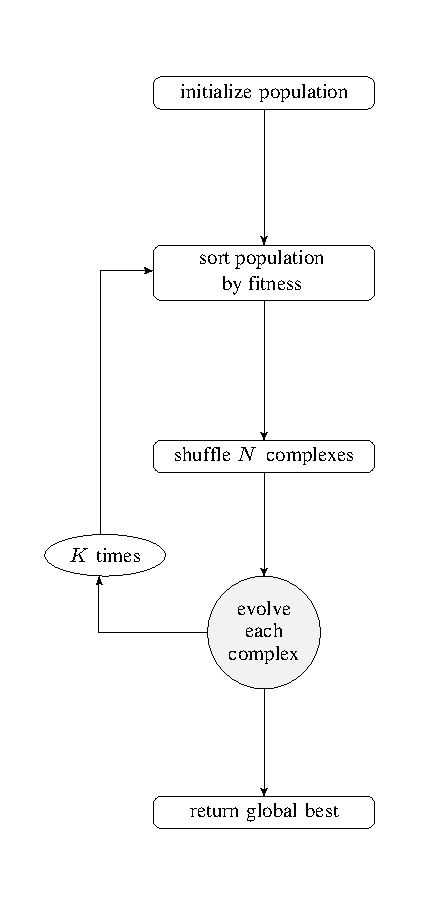
\includegraphics[width=0.47\linewidth]{imgs/flow1}
    \label{fig:flow1}
  }
  ~
  \subfigure[Evolving stage for a single complex.]{
    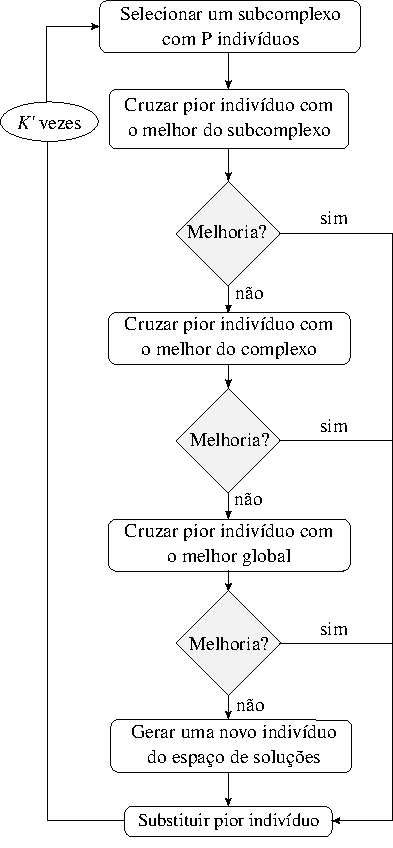
\includegraphics[width=0.47\linewidth]{imgs/flow2}
    \label{fig:flow2}
  }
  \caption{Flowchart representing the shuffled complex evolution algorithm.}
  \label{fig:sce}
\end{figure}


\subsection{The shuffled complex evolution for the MKP}

As it can be noted in its description the SCE is easly applied to any
optimization problem.
The only steps needed to be specified is (a) the creation of a new random
solution and (b) the crossing procedure of two solutions.
These two procedures are respectively presented by Algorithm.~\ref{alg:new} and
Algorithm~\ref{alg:cross}.

\begin{algorithm}
\begin{algorithmic}[1]
  \Procedure{New random solution}{}
    \State $v \leftarrow $ shuffle($1, 2, \ldots, n$)
	\State $s \leftarrow \emptyset$ \Comment{empty solution}
    \For{$ i \leftarrow 1:n$ }
	  \State $s \leftarrow s \cup \{v_i\}$ \Comment{adding item}
	  \If{ $s$ is not feasible} \Comment{checking feasibility}
	    \State $s \leftarrow s - \{v_i\}$
      \EndIf
	\EndFor
  \State return $s$
  \EndProcedure
\end{algorithmic}
\caption{Generation of a new random solution for the MKP.}
\label{alg:new}
\end{algorithm}

To construct a new random solution (Algorithm~\ref{alg:new}) the items are
at first shuffled in random order and stored in a list (line 2).
A new empty solution is then defined (line 3).
The algorithm iteratively tries to fill the solution's knapsack with 
the an item taken from the list (lines 4-9).
The feasibility of the solution is then checked: if the item insertion let
the solution unfeasible (line 6) its removed from knapsack (line 7).
After trying to place all available items the new solution is returned.

The crossing procedure (Algorithm~\ref{alg:cross}) takes as input the worst
solution taken from the subcomplex $x^w = (x^w_1, x^w_2, \ldots, x^w_n$),
the selected better solution $x_b = (x^b_1, x^b_2, \ldots, x^b_n$)
and the number $c$ of genes that will be carried from the better solution.
The $c$ parameter will control how similar the worst individual will be from the
given better individual.
At first the items are shuffled in random order and stored in a list (line 2).
Then $c$ randomly chosen genes are carried from the better individual to the worst
individual (line 5).
At the end of steps the feasibility of the solution is checked (line 7) and
the solution is repaired if needed.
The repair stage is a greedy procedure that iteratively removes the item that less
decreases the objective function.
Finally the fitness of the generated solution is updated (line 10) and
returned (line 11).

\begin{algorithm}[t]
\begin{algorithmic}[1]
  \Procedure{Crossing}{$x^w:$ worst individual, $x^b:$ better individual, $c$}
    \State $v \leftarrow $ shuffle($1, 2, \ldots, n$)
    \For{$ i \leftarrow 1:c$ }
	  \State $j \leftarrow v_i$
	  \State $x^w_j \leftarrow x^b_j$ \Comment{gene carriage}
	\EndFor
	\If{$s^w$ is not feasible}
	  \State repair $s^w$
	\EndIf
	\State update $s^w$ fitness
  \State return $s^w$
  \EndProcedure
\end{algorithmic}
\caption{Crossing procedure used on SCE algorithm.}
\label{alg:cross}
\end{algorithm}

%\begin{algorithmic}
%  \Procedure{The SCE for the MKP}{$\vec{p}, W, \vec{b}$}
%    \State Inicialize population
%    \For{$ i \leftarrow 1:K$ }
%	  \State Sort population by fitness
%	  \State $s_{gb} \leftarrow$ Global best individual
%	  \State Shuffle complexes
%      \For{ each complex }
%	    \State $s_{cb} \leftarrow$ Complex best individual
%        \For{$ k \leftarrow 1:K'$ }
%		  \State Select a subcomplex of $P$ individuals
%          \State $s_w \leftarrow$ worst individual of subcomplex
%          \State $s_b \leftarrow$ best individual of subcomplex
%		  \State $s_{new} \leftarrow s_w \otimes s_b$
%		  \If{ $fitness(s_{new}) > s_w$}
%		    \State $s_w \leftarrow s_{new}$
%		  \Else
%		    \State $s_{new} \leftarrow s_w \otimes s_{cb}$
%		    \If{ $fitness(s_{new}) > s_w$}
%		      \State $s_w \leftarrow s_{new}$
%			\Else
%		      \State $s_{new} \leftarrow s_w \otimes s_{gb}$
%		      \If{ $fitness(s_{new}) > s_w$}
%		        \State $s_w \leftarrow s_{new}$
%		      \Else
%			    \State $s_w \leftarrow$ new random solution
%			  \EndIf
%		    \EndIf
%		  \EndIf
%        \EndFor
%      \EndFor
%    \EndFor
%	\State $s_gb \leftarrow$ Global best individual
%	\State Return $s_gb$
%  \EndProcedure
%\end{algorithmic}

%\begin{algorithmic}
%  \Procedure{New random MKP solution}{$\vec{p}, W, \vec{b}$}
%    \State $\vec{v} \leftarrow $ shuffle$(1, 2, \ldots, n)$
%	\State $s \leftarrow \emptyset $
%    \For{$ i \leftarrow 1:niter$ }
%	  \If{$ s \cup \{v[i]\} is feasible$}
%	    \State $s \leftarrow s \cup \{v[i]\}$
%	  \EndIf
%    \EndFor
%  \EndProcedure
%\end{algorithmic}
